\chapter{طراحی یک پلتفرم \lr{MLOps}}
 
\section{مقدمه}
در این بخش می خواهیم مقدمه ای از طراحی و هدف آن بنویسیم

\section{سیستم مدیریت پلتفرم}
\subsection{مدیریت پیکربندی و فراهم سازی زیرساخت}
در دنیای فناوری اطلاعات، زیرساخت‌های تغییرناپذیر\footnote{\lr{Immutable Infrastructure}} و تغییرپذیر\footnote{\lr{Mutable Infrastructure}} دو رویکرد مهم در مدیریت و نگهداری سیستم‌ها هستند. زیرساخت‌های تغییرناپذیر به سیستم‌هایی اشاره دارند که پس از ایجاد، بدون تغییر باقی می‌مانند و در صورت نیاز به تغییر، سیستم های جدید جایگزین آنها می‌شوند. این رویکرد با مزایایی همچون کاهش پیچیدگی‌های مدیریتی، افزایش قابلیت پیش‌بینی و کاهش ریسک‌های مرتبط با تغییرات ناخواسته همراه است \cite{DevopsIaac2}. به کمک ابزارهایی مانند داکر و کوبرنتیز، پیاده‌سازی زیرساخت‌های تغییرناپذیر امکان‌پذیر است و از قابلیت مقیاس‌پذیری بالایی برخوردارند. سیستم‌های ابری غالباً از روش تغییرناپذیر استفاده کرده تا از مزایای آن بهره‌مند شوند. در مقابل، زیرساخت‌های تغییرپذیر به سیستم‌هایی اشاره دارند که می‌توانند به طور پویا تغییر کنند و تنظیمات و پیکربندی‌های جدید را بپذیرند. این رویکرد، انعطاف‌پذیری بیشتری را فراهم می‌کند و برای محیط‌هایی که نیاز به تغییرات مکرر دارند، مناسب‌تر است. با این حال، مدیریت تغییرات در زیرساخت‌های تغییرپذیر ممکن است چالش‌های بیشتری از جمله افزایش ریسک خطاها و نیاز به نظارت مداوم به همراه داشته باشد. انتخاب بین این دو رویکرد به نیازها و اولویت‌های سازمان بستگی دارد. در حالی که زیرساخت‌های تغییرناپذیر برای محیط‌های تولید با نیاز به ثبات و قابلیت پیش‌بینی بالا مناسب‌ترند، زیرساخت‌های تغییرپذیر برای محیط‌های توسعه و آزمایش که نیاز به انعطاف‌پذیری دارند، کاربرد بیشتری دارند \cite{DevopsIaac1}. این دو مفهوم به صورت مستقیم با مدیریت پیکربندی وفراهم سازی زیرساخت مرتبط هستند.
\subsubsection{مدیریت پیکربندی}
مدیریت پیکربندی فرآیندی است که بر روی نگهداری و کنترل پیکربندی سیستم‌ها و نرم‌افزارها تمرکز دارد. هدف اصلی این فرآیند، اطمینان از سازگاری و پایداری محیط‌های \lr{IT} در طول زمان است. مدیریت پیکربندی شامل فعالیت‌هایی مانند نگهداری نسخه‌های مختلف نرم‌افزار، مستندسازی تغییرات و اطمینان از تطابق سیستم‌ها با استانداردهای تعیین شده می‌باشد. ابزارهای مدیریت پیکربندی مانند \lr{Ansible} و \lr{Puppet} به سازمان‌ها کمک می‌کنند تا فرآیندهای خودکارسازی پیکربندی را پیاده‌سازی کنند. این ابزارها از فایل‌های متنی (مانند \lr{Playbook}ها در \lr{Ansible}) برای تعریف وضعیت مطلوب سیستم‌ها استفاده می‌کنند. \lr{Ansible} \cite{Ansible} به دلیل سادگی و عدم نیاز به نصب عامل\footnote{\lr{Agent}} بر روی سیستم‌های مقصد، یکی از محبوب‌ترین ابزارهای مدیریت پیکربندی است. این ابزار از پروتکل \lr{SSH} برای ارتباط با ماشین‌ها استفاده می‌کند و از زبان \lr{YAML} برای نوشتن اسکریپت‌ها بهره می‌برد، که خوانایی و قابل فهم بودن آن را تضمین می‌کند. از ابزار های مدیریت پیکربندی در زیرساخت های تغییرپذیر غالبا استفاده می شود.

\subsubsection{فراهم سازی زیرساخت}
فراهم سازی زیرساخت فرآیندی است که به راه‌اندازی و پیکربندی اولیه زیرساخت‌های \lr{IT} اختصاص دارد. این فرآیند شامل ایجاد و مدیریت منابعی مانند سرورها، پایگاه داده‌ها، شبکه‌ها و سایر اجزای زیرساختی است. فراهم سازی زیرساخت به صورت سنتی فرآیندی دستی و زمان‌بر بود، اما با ظهور ابزارهای نوین این فرآیند به شدت خودکار و ساده شده است. ابزارهای متن بازی مانند \lr{Terraform} برای این کار استفاده می‌شوند. این ابزارها به کاربران امکان می‌دهند تا زیرساخت‌های خود را به صورت کد\footnote{\lr{Infrastructure as Code}} تعریف کنند \cite{DevopsIaac1}. این رویکرد به ایجاد و مدیریت منابع زیرساختی به صورت قابل تکرار و پایدار کمک می‌کند. \lr{Terraform}، یکی از پرکاربردترین ابزارهای فراهم سازی زیرساخت، از زبان \lr{HCL} برای تعریف زیرساخت‌ها استفاده می‌کند. یکی از ویژگی‌های برجسته \lr{Terraform} مدیریت وابستگی‌ها بین منابع است که امکان بازگردانی\footnote{\lr{Rollback}} به وضعیت‌های قبلی را نیز فراهم می‌کند \cite{Terraform}. از این ابزار ها غالبا برای زیرساخت ها تغییرناپذیر استفاده می شود.

در زیرساخت طراحی شده که از \lr{OpenStack} برای ساخت و مدیریت ماشین های مجازی استفاده می شود، استفاده از \lr{Ansible} به عنوان ابزار مدیریت پیکربندی به دلایل متعددی مناسب است. اولاً، \lr{Ansible} با استفاده از \lr{Playbook}های \lr{YAML} امکان خودکارسازی مراحل پیکربندی را فراهم می‌کند، از جمله نصب نرم‌افزارهای مورد نیاز، تنظیمات شبکه و پیکربندی سرویس‌ها. این ویژگی باعث می‌شود که پیکربندی‌ها به صورت دقیق و بدون خطا انجام شود. ثانیاً، \lr{Ansible} بدون نیاز به نصب عامل  بر روی ماشین های مجازی کار می‌کند و از پروتکل \lr{SSH} برای ارتباط استفاده می‌کند که این امر فرآیند پیکربندی را ساده‌تر و سریع‌تر می‌سازد. همچنین، تمامی مراحل پیکربندی به صورت کد تعریف می‌شوند که امکان اجرای مجدد و دقیق همان تنظیمات را بر روی ماشین‌های جدید فراهم می‌کند. به علاوه، \lr{Ansible} دارای ماژول‌های متعددی برای تعامل با \lr{OpenStack} است که می‌تواند فرآیند ایجاد و مدیریت ماشین های مجازی را بهینه‌تر کند. پس از پیکربندی اولیه \lr{VM}ها، \lr{Ansible} می‌تواند خوشه کوبرنتیز را به صورت خودکار راه‌اندازی و پیکربندی کند. این شامل نصب ابزارهای مورد نیاز، تنظیمات شبکه و پیکربندی سرویس‌های کوبرنتیز است.
\subsection{خط لوله \lr{CI/CD}}
با افزایش استفاده از سیستم‌های ابری و رویکرد تغییرناپذیر، مفهومی با عنوان \lr{GitOps} معرفی شد که از گیت برای مدیریت زیرساخت و پیکربندی بهره می‌برد. \lr{GitOps} توسط \lr{Weaveworks} در سال ۲۰۱۷ معرفی شد که رویکردی مدرن برای پیاده سازی خط لوله \lr{CD} بر روی سیستم های ابری است. در حالی که ابزارهای سنتی تحویل مداوم عمدتاً از مدل \lr{Push} استفاده می‌کنند، \lr{GitOps} مدل \lr{Pull} را معرفی می‌کند که به خصوص با کانتینرها و پیکربندی‌های اعلامی به خوبی کار می‌کند و آن را به یک روند محبوب در اکوسیستم بومی ابر تبدیل کرده است  \cite{Devopsgitops}. از معروف ترین ابزار کلیدی که فرآیندهای \lr{GitOps} را تسهیل می‌کند می توان به \lr{ArgoCD} اشاره کرد. 



\begin{figure}[t]
	\centering
	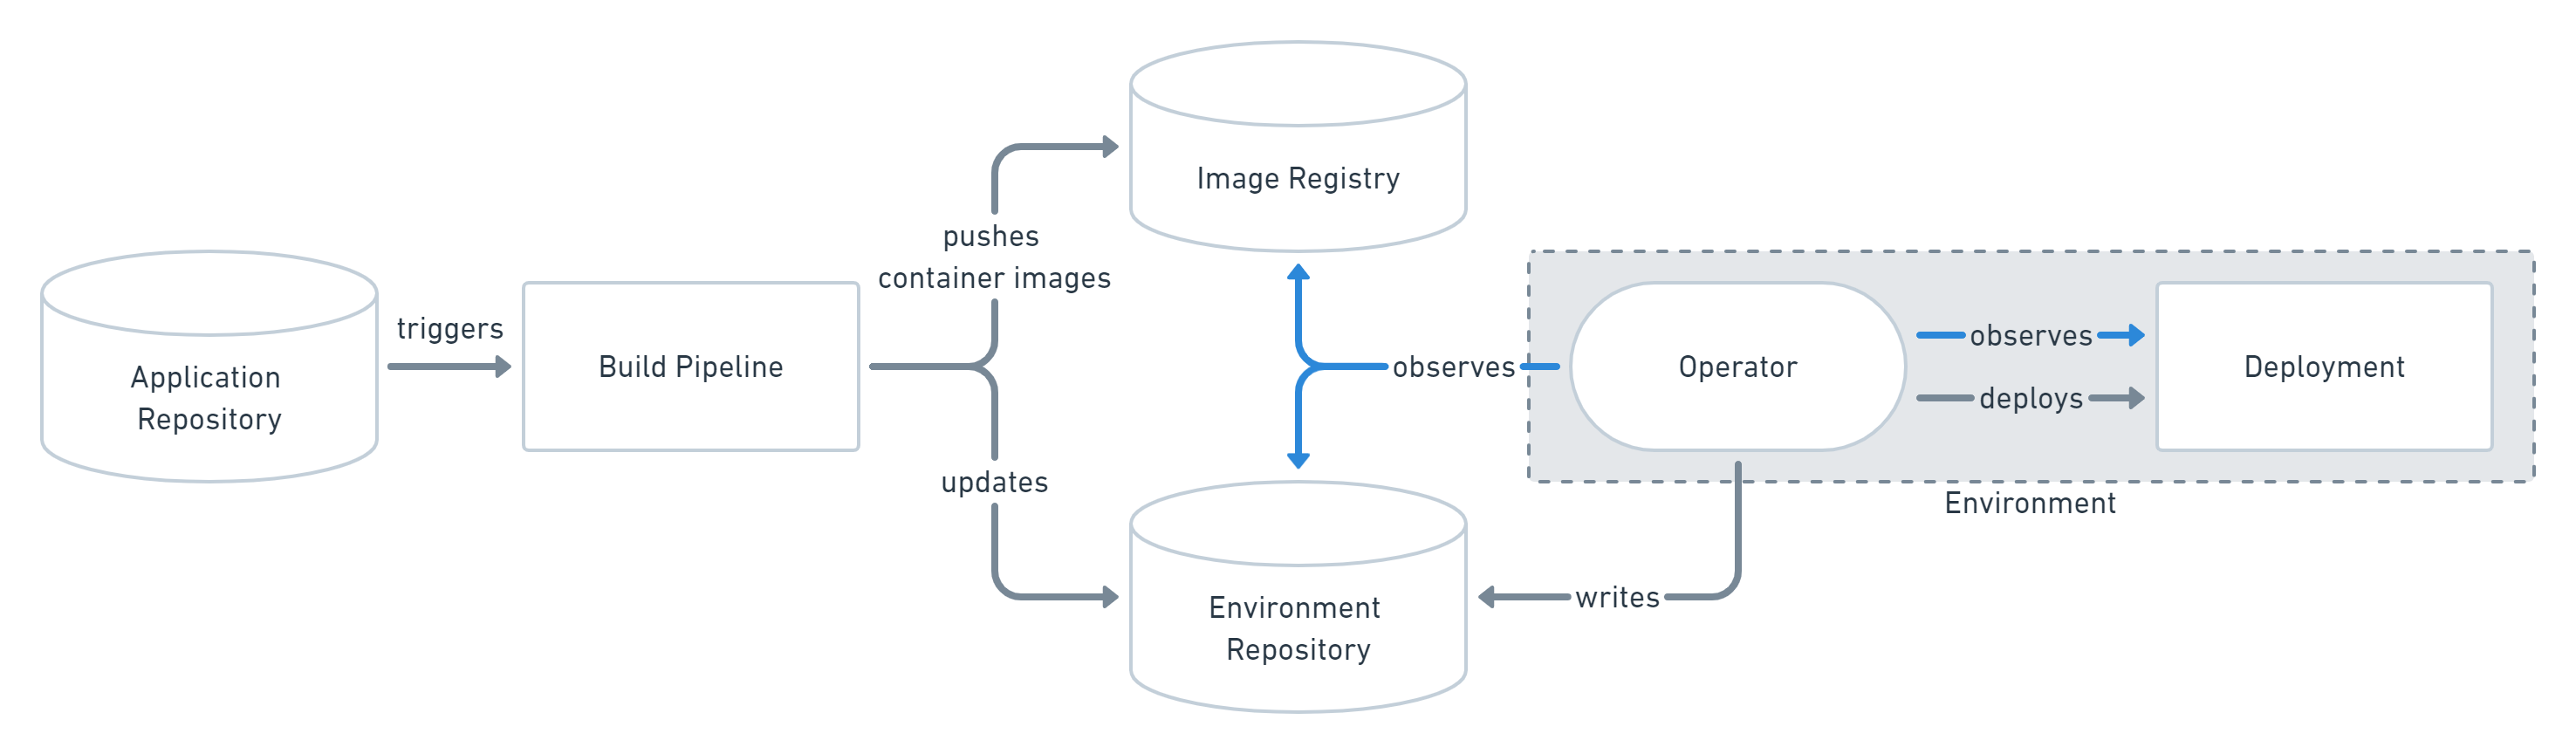
\includegraphics[scale=0.15]{gitops-pull.png}
	\caption{استقرار مبتنی بر \lr{Pull}}
	\label{fig: gitops pull}
\end{figure}

همان طور که گفته شد دو رویکرد در پیاده سازی خط لوله \lr{CD} وجود دارد. در مدل \lr{Pull} 
(شکل 
~\ref{fig: gitops pull})
مانند \lr{GitOps}، توسعه‌دهندگان حالت مطلوب را در مخزن گیت قرار می دهند. ابزاری نظیر \lr{ArgoCD} در محیط تولید به صورت خودکار این تغییرات را شناسایی کرده و اعمال می‌کنند. این مدل امنیت را افزایش می‌دهد زیرا نیازی به اعتبارنامه‌های دسترسی مستقیم برای توسعه‌دهندگان نیست. هم چنین این مدل مشکل استقرارهای مبتنی بر \lr{Push} را حل می کند، که در آن محیط تنها زمانی به روز می شود که مخزن محیط به روز شود. 
در مقابل، در مدل \lr{Push} (شکل 
~\ref{fig: gitops push})، استقرار در محیط تولید شامل خطوط لوله \lr{CI/CD} با اسکریپت‌هایی است که با هر تغییر در گیت فعال می‌شوند. این اسکریپت‌ها معمولاً ساخت، تست و در نهایت استقرار برنامه‌ها یا تنظیم پیکربندی‌های جدید در محیط تولید را با استفاده از ابزارهای خط فرمان و اعتبارنامه‌های ارائه شده انجام می‌دهند. این مدل کنترل دقیق‌تر بر فرآیند استقرار، اعمال سریع تغییرات، انعطاف‌پذیری بالا در مدیریت سناریوهای پیچیده و پشتیبانی بهتر از تغییرات جزئی را فراهم می‌کند، که در محیط‌های متنوع و پویا بسیار مفید است \cite{Devopsgitops}.
\begin{figure}[t]
	\centering
	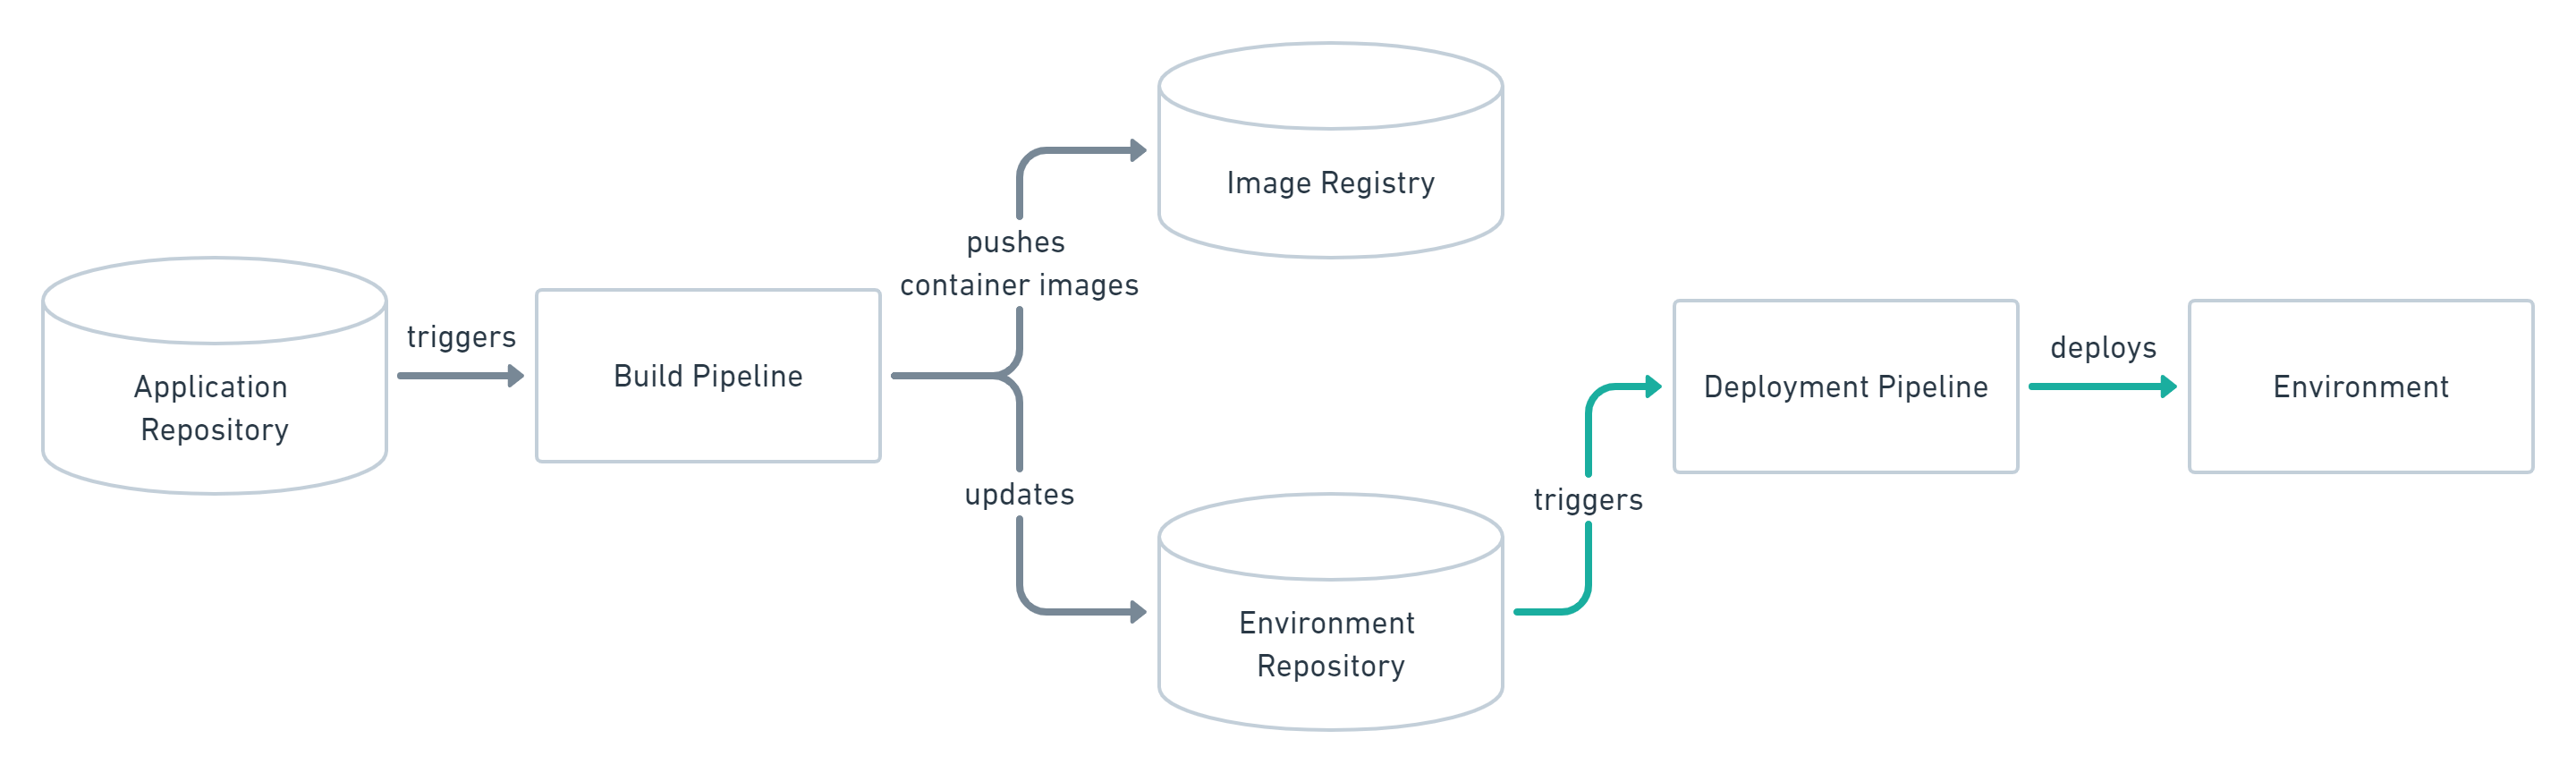
\includegraphics[scale=0.15]{gitops-push.png}
	\caption{استقرار مبتنی بر \lr{Push}}
	\label{fig: gitops push}
\end{figure}

به منظور پیاده‌سازی یک ابزار متن‌باز برای مدیریت خط لوله های \lr{CI/CD} که برای سیستم‌های ابری نیز مناسب باشد،  رویکرد تغییرپذیر  به همراه استراتژی استقرار مبتنی بر \lr{Push} انتخاب شده است. انتخاب رویکرد تغییرپذیر به دلیل نیاز به انعطاف‌پذیری بیشتر در محیط‌هایی که تغییرات مکرر و به‌روزرسانی‌های سریع دارند، انجام شده است. زیرساخت‌های تغییرپذیر به ما امکان می‌دهند تا به سرعت به تغییرات نیازمندی‌ها، پاسخ دهیم و تنظیمات و پیکربندی‌های جدید را به راحتی اعمال کنیم. این ویژگی در محیط‌های توسعه و آزمایش بسیار حیاتی است، زیرا تغییرات مداوم و آزمایش‌های متعدد بخشی از فرآیند توسعه نرم‌افزار هستند. هم چنین روش \lr{Push} نیز به دلیل سادگی و کارایی در اعمال به‌روزرسانی‌ها انتخاب شده است. با استفاده از این روش، می‌توانیم به‌روزرسانی‌ها را مستقیماً به سرورها ارسال کنیم و اطمینان حاصل کنیم که تمام سیستم‌ها به سرعت و بدون نیاز به مداخله دستی به‌روز می‌شوند. این رویکرد همچنین به کاهش زمان مورد نیاز برای انتشار تغییرات کمک می‌کند. در این راستا، \lr{Jenkins} به عنوان ابزار پیاده‌سازی و مدیریت خط لوله \lr{CI/CD} انتخاب شده است. جنکینز به دلیل متن‌باز بودن و دارا بودن تعداد زیادی پلاگین، انعطاف‌پذیری بسیار بالایی دارد و می‌تواند با انواع سیستم‌های ابری و رویکردهای زیرساختی سازگار شود. جنکینز همچنین با \lr{Ansible} که به عنوان ابزار مدیریت پیکربندی انتخاب شد، به خوبی سازگار است. این ترکیب به ما اجازه می‌دهد تا پیکربندی‌های پیچیده را به سادگی مدیریت کنیم و اطمینان حاصل کنیم که تمام زیرساخت‌ها به صورت هماهنگ عمل می‌کنند.
\subsubsection{طراحی خط لوله}
؟?????????
\subsection{مخزن کد منبع}

مخزن کد منبع\footnote{\lr{Source Code Repository}} یک سیستم ذخیره‌سازی و مدیریت کد است که به توسعه‌دهندگان این امکان را می‌دهد تا به صورت مشترک و هماهنگ بر روی پروژه‌های نرم‌افزاری کار کنند. این مخازن ابزارهای متعددی را برای تسهیل و بهبود فرآیند توسعه نرم‌افزار فراهم می‌کنند. یکی از اصلی‌ترین ویژگی های مخزن کد منبع، کنترل نسخه است که به توسعه‌دهندگان این امکان را می‌دهد تا تغییرات کد را پیگیری کرده و به نسخه‌های قبلی بازگردند. این ابزارها با ثبت تاریخچه تغییرات و شاخه‌بندی، امکان مدیریت همزمان چندین ویژگی یا رفع اشکال را فراهم می‌کنند بدون اینکه تغییرات یکدیگر را تحت تأثیر قرار دهند.

رایج‌ترین و پرکاربردترین این مخازن، گیت است که با ابزارهای مختلفی مانند \lr{GitHub}، \lr{GitLab} و \lr{Bitbucket} یکپارچه می‌شود. از آنجایی که یکی از شرط های پیاده سازی پلتفرم، متن باز بودن ابزار های آن می باشد، \lr{GitLab} برای مدیریت مخزن کد منبع استفاده شده است. در این طراحی \lr{Jenkins} به \lr{GitLab} به عنوان مخزن کد متصل شده و هر تغییر در کد منبع باعث اجرا شدن یک خط لوله \lr{CI/CD} مشخص توسط \lr{Jenkins} می گردد.

\subsection{مخزن مؤلفه ها}
یک مخزن مؤلفه\footnote{\lr{Artifact Repository}} یک سیستم متمرکز برای ذخیره‌سازی، مدیریت و انتشار مؤلفه های نرم‌افزاری است. این مؤلفه ها شامل هر نوع فایل باینری، کتابخانه، ماژول، پکیج، پلاگین یا حتی مستنداتی می‌شود که در طول چرخه عمر توسعه نرم‌افزار تولید می‌شود. هدف اصلی این مخازن این است که به تیم‌های توسعه اجازه دهد تا به راحتی نسخه‌های مختلفی از مؤلفه ها را مدیریت و به اشتراک بگذارند، فرآیندهای ساخت و انتشار را ساده کنند و وابستگی‌ها را طور موثرتری مدیریت کنند. همچنین، از انتشار مؤلفه هایی که هنوز تست نشده‌اند یا از نظر امنیتی مشکلاتی دارند جلوگیری می‌کنند. 
یکی از ابزارهای محبوب و متن باز برای مدیریت مخازن مؤلفه ها، \lr{Nexus} است. \lr{Nexus} از فرمت‌های مختلف مؤلفه ها مانند \lr{Helm}، \lr{apt}، \lr{PyPI} و \lr{Docker} پشتیبانی می‌کند، که این امر آن را به یک ابزار چندمنظوره برای انواع پروژه‌های نرم‌افزاری تبدیل می‌کند. مخازن مؤلفه موردنیاز برای پیاده سازی پلتفرم در 4 نوع \lr{raw}، \lr{apt}، \lr{PyPI} و \lr{Docker} می باشد.

\subsubsection{مخازن \lr{APT}}
یک سیستم مدیریت بسته در سیستم‌عامل‌های مبتنی بر دبیان است که به کاربران اجازه می‌دهد تا بسته‌های نرم‌افزاری را به راحتی نصب، به‌روزرسانی و حذف کنند. از آنجایی بسته های استفاده شده در سرور ها غالبا یکسان می باشد، به منظور افزایش سرعت پیاده سازی و اعمال تغییرات و پیکربندی تمامی بسته های مورد استفاده و نصب نشده در محیط، در \lr{Nexus} ذخیره خواهند شد. این امر با استفاده از مخازنی از نوع \lr{Proxy} انجام خواهد شد. در پیاده سازی سیستم علاوه بر بسته های موجود در \lr{APT} رسمی \lr{Ubuntu}، از مخازن \lr{Containerd} و \lr{Kubernetes} نیز برای نصب و پیاده سازی کوبرنتیز نیز استفاده شده است. علاوه بر این، یک مخزن هم برای نصب \lr{Nvidia Driver} و \lr{Nvidida CUDA Toolkit} برای استفاده از واحد پردازنده گرافیکی ایجاد خواهد شد.
\subsubsection{مخزن \lr{PyPI}}
	یک مخزن عمومی برای بسته‌های نرم‌افزاری پایتون است که به توسعه‌دهندگان اجازه می‌دهد تا کتابخانه‌ها و ابزارهای خود را منتشر، به‌روزرسانی و مدیریت کنند. کاربران می‌توانند این بسته‌ها را به‌راحتی با استفاده از ابزار \lr{pip} نصب کنند. همانند \lr{APT}، به منظور ذخیره سازی تمامی بسته های استفاده شده در محیط تولید ساخته شده اند. این امر باعث افزایش سرعت در نصب مجدد بسته ها و پایداری سیستم در زمان های قطعی یا خرابی مخازن رسمی می شود.
\subsubsection{مخزن \lr{Docker}}
	یک سرویس برای \lr{Docker Images} است که به توسعه‌دهندگان اجازه می‌دهد تا تصاویر خود را ذخیره، مدیریت و به اشتراک بگذارند. با توجه به تحریم استفاده از \lr{DockerHub} در ایران وهم چنین کند بودن راه های جایگزین در گرفتن تصاویر موردنظر از مخازن رسمی این مخزن به وجود آمده که به مخزن رسمی \lr{docker.io} پراکسی شده است. علاوه بر این تصاویر لازم برای پیاده سازی و پیکربندی محیط که با خط لوله \lr{CI/CD} ساخته شده اند نیز برای استفاده مجدد در این مخازن قرار می گیرند.
\subsubsection{مخزن \lr{raw}}
	برای ذخیره‌سازی و مدیریت فایل‌ها و داده‌هایی استفاده می‌شود که فرمت خاصی ندارند. این نوع مخزن به توسعه‌دهندگان اجازه می‌دهد تا انواع مختلف فایل‌ها، مانند اسکریپت‌ها، تصاویر، و مستندات را بدون نیاز به ساختاردهی خاصی نگهداری کنند.


شکل از نکسوس بگذار ؟؟؟؟؟؟؟؟؟؟؟؟؟؟؟؟؟؟؟؟؟؟؟؟؟؟؟؟؟؟؟؟؟؟؟؟؟؟؟؟؟؟؟؟؟؟؟؟؟؟؟










